\documentclass[11pt,a4paper]{article}
\usepackage[T1]{fontenc}
\usepackage{lmodern}
\usepackage[margin=2.5cm]{geometry}
\usepackage{amsmath,amssymb}
\usepackage{booktabs}
\usepackage{array}
\usepackage{enumitem}
\usepackage{xcolor}
\usepackage{graphicx}
\graphicspath{{../figures/}}
\PassOptionsToPackage{hyphens}{url}
\usepackage[colorlinks=true,linkcolor=blue!50!black,urlcolor=blue!50!black]{hyperref}

\renewcommand{\Re}{\operatorname{Re}}
\renewcommand{\Im}{\operatorname{Im}}
\newcommand{\dext}{\delta_{\rm ext}}
\newcommand{\Lop}{\mathcal{L}_\ell}
\newcommand{\x}{\mathbf{x}}
\newcommand{\code}[1]{\texttt{#1}}
\newcommand{\PhiP}{\Phi^{\rm P}}
\newcommand{\PhiR}{\Phi^{\rm R}}
\newcommand{\Pres}{\Phi^{\rm res}}
\newcommand{\lpm}{{\ell'_{\max}}}

\title{Complex-contour regularisation of the massive scalar toy model\\[4pt]
\large Truncated punctures, Bessel homogeneous solutions and the angular quadrature with an exponential}
\author{Draft prepared with Claude Code for Andrew Spiers (UCD)}
\date{25 October 2026}

\begin{document}
\maketitle

\begin{abstract}
The complex-contour regularisation of second-order point-particle sources, developed on the massless scalar toy model, is tested on the massive (screened Poisson) model $(\nabla^2-m^2)\Phi_2=\tfrac12\partial_Z^2(\Phi_1^2)$ with $mr_0=1$ and $5$.
The model removes three conveniences of the massless case at once: the singular field $qe^{-m\rho}/\rho$ is an infinite local series and punctures must be truncated; the homogeneous mode solutions are modified spherical Bessel functions; and the SS source's $\rho$-integrand is an entire function times a Laurent polynomial.
With a reference built mode by mode from closed-form source modes and verified four independent ways to $10^{-18}$ or better, we find: the complex-radius angular quadrature still works with the same node count once the two branches are blended with the continued step and the in-branch logarithm is placed on the same side of the cut as the out-branch, reproducing the closed-form continuation to $8\times10^{-15}$; the consistency conditions on the continued singular mode behave exactly as in the massless case, with a purely imaginary residual $\tfrac i\pi E_0$, $E_0(r_0)=-1/r_0$ for every $\ell$ and $m$; the exterior second-order field with the exact puncture is recovered to $5\times10^{-18}$ ($mr_0=1$) and $9\times10^{-17}$ ($mr_0=5$) with no spurious worldline terms; and with punctures truncated at $\rho^n$ the hybrid split converges as $\lpm^{-(n+4)}$ (fitted slopes $4.87$, $6.82$, $8.78$ for $n=1,3,5$), two orders faster than the massless $cq\rho^n$ trick because the first omitted term is an even power of $\rho$.
Two features are new: the SS source carries a $\delta$-function term, $4\pi mq^2Y_\ell(0)/r_0^2$, from the constant $-mq$ of the singular field, and one branch of the angular quadrature is no longer enough.
At $m=0$ every stage reproduces the massless results.
\end{abstract}

{\small\tableofcontents}

\section{Why a massive model}\label{sec:why}
The complex-contour method of the massless note and PRD draft was developed on the flat-space Poisson toy model, where the first-order singular field is the Coulomb potential $q/\rho$, the homogeneous solutions of every mode equation are the powers $r^\ell$ and $r^{-\ell-1}$, and the singular field is a finite closed form because the injected regular field is a polynomial.
None of these conveniences survives in gravity.
A gravitational puncture is an infinite local series in the distance $\rho$ that must be truncated; the homogeneous solutions of the Regge--Wheeler, Lorenz-gauge or Teukolsky equations are special functions; and the regular field is a solution of the homogeneous field equation, not of Laplace's equation.

The screened Poisson equation, $(\nabla^2-m^2)\Phi=S$, is the simplest model that removes all three conveniences at once while keeping everything else of the massless test intact.
\begin{itemize}[leftmargin=*]
\item The singular field $q\,e^{-m\rho}/\rho=q(\rho^{-1}-m+\tfrac12m^2\rho-\tfrac16m^3\rho^2+\dots)$ is an infinite series, so punctures must be truncated at some order $\rho^n$ exactly as in gravity, and the second-order field converges algebraically with the coupled-mode cutoff $\lpm$ at a rate set by the order of truncation (test T1).
\item The homogeneous mode solutions are the modified spherical Bessel functions $i_\ell(mr)$ and $k_\ell(mr)$, so the continued singular mode, the $\Theta\to H$ blend of kinked modes, the consistency conditions of PRD App.~C and the physical boundary conditions at the ends of the domain all have to be rebuilt with non-polynomial functions (test T3).
\item The singular--singular source $\tfrac12\partial_Z^2(q^2e^{-2m\rho}/\rho^2)$ is still a closed-form function of position, so the complex-radius angular quadrature in the distance $\rho$ applies, but its $\rho$-integrand is no longer a Laurent polynomial: it is a Laurent polynomial times an entire function (test T2).
\end{itemize}
The parameter $m r_0$ measures how far the model is from the massless one; we use $mr_0=1$ and $5$, i.e.\ $m=\tfrac15$ and $m=1$ at $r_0=5$, and $m=0$ as a check that everything reduces to the massless results.
Throughout, $Z=r\mu$ denotes the Cartesian coordinate along the symmetry axis and $z$ the complexified radial coordinate.

\section{The model and its exact reference}\label{sec:model}

\subsection{First order}
The first-order field satisfies $(\nabla^2-m^2)\Phi_1=-4\pi q\,\delta^3(\x-\x_0)$ with $\x_0=r_0\hat Z$, so
\begin{equation}
\Phi_1=\frac{q\,e^{-m\rho}}{\rho}+\PhiR_1,\qquad (\nabla^2-m^2)\PhiR_1=0 ,
\end{equation}
where the regular field is injected through the boundary data and is regular at the origin.
We take
\begin{equation}
\PhiR_1=c_0\,\frac{u_0(r)}{u_0(r_0)}+c_1r_0\,\frac{u_1(r)}{u_1(r_0)}\,\mu,\qquad c_0=1,\ c_1=\tfrac1{10},
\label{eq:phiR}
\end{equation}
which has $\PhiR_1(\x_0)=c_0+c_1r_0=\tfrac32$ for every $m$ and reduces to the massless $c_0+c_1Z$ as $m\to0$.
Here $u_\ell$ and $v_\ell$ are the homogeneous solutions of the mode operator
\begin{equation}
\Lop\psi=\psi''+\frac2r\psi'-\Big[\frac{\ell(\ell+1)}{r^2}+m^2\Big]\psi,
\end{equation}
normalised so that they tend to the massless powers,
\begin{gather}
u_\ell(r)=\frac{(2\ell+1)!!}{m^\ell}\,i_\ell(mr)\to r^\ell,\qquad
v_\ell(r)=\frac{m^{\ell+1}}{(2\ell-1)!!}\,k_\ell(mr)\to r^{-\ell-1},\nonumber\\
u_\ell v_\ell'-u_\ell'v_\ell=-\frac{2\ell+1}{r^2},
\label{eq:uv}
\end{gather}
with $i_\ell(x)=\sqrt{\pi/2x}\,I_{\ell+1/2}(x)$ and $k_\ell(x)=\sqrt{2/\pi x}\,K_{\ell+1/2}(x)$.
With this normalisation every massless formula carries over by the replacement $r_<^\ell/r_>^{\ell+1}\to u_\ell(r_<)v_\ell(r_>)$: the Green's function with the physical conditions (regular at the origin, decaying at infinity) is $G_\ell(r,s)=-(s^2/(2\ell+1))\,u_\ell(r_<)v_\ell(r_>)$, the massive Coulomb mode is
\begin{equation}
\Big[\frac{q\,e^{-m\rho}}{\rho}\Big]_L=q\sqrt{\frac{4\pi}{2L+1}}\;u_L(r_<)\,v_L(r_>),
\label{eq:coulomb}
\end{equation}
and the jump of its derivative at $r_0$, $-\sqrt{4\pi(2L+1)}/r_0^2$, is independent of $m$.
Equation~\eqref{eq:coulomb} was checked in three ways (direct angular quadrature, the Bessel form, and the $\rho$-substitution closed form of Sec.~\ref{sec:ssmodes}) to $10^{-41}$.
The physical boundary conditions are imposed as Robin conditions, $\psi'=\psi\,u_\ell'/u_\ell$ at $r=1$ and $\psi'=\psi\,v_\ell'/v_\ell$ at $r=10$, which the Green's function satisfies exactly.

\subsection{Second order and the exact reference}\label{sec:reference}
The second-order field satisfies $(\nabla^2-m^2)\Phi_2=\tfrac12\partial_Z^2(\Phi_1^2)$, and because $\partial_Z$ commutes with the screened operator, $\Phi_2=\tfrac12\partial_Z^2\chi$ with $(\nabla^2-m^2)\chi=\Phi_1^2$.
Unlike the massless case $\chi$ is not closed form in three dimensions.
Its SS part is: writing $u=\rho\chi$ for the spherically symmetric part, $u''-m^2u=q^2e^{-2m\rho}/\rho$ gives
\begin{align}
\chi_{\rm SS}&=q^2\bigg[\frac{e^{m\rho}\,{\rm Ei}(-3m\rho)-e^{-m\rho}\,{\rm Ei}(-m\rho)}{2m\rho}-\frac{\ln3}{2m}\,\frac{\cosh m\rho}{\rho}\bigg]\nonumber\\
&=q^2\ln\rho+q^2\Big(\gamma+\ln m+\tfrac12\ln3-1\Big)+O(\rho\ln\rho),
\label{eq:chiSS}
\end{align}
where the homogeneous term $\cosh(m\rho)/\rho$ removes the $1/\rho$ piece of the particular solution so that no point source sits at $\x_0$; the remaining freedom, $\sinh(m\rho)/\rho$, is entire and is absorbed by the boundary conditions.
The SR and RR parts involve products of Bessel functions and have no elementary particular solution.

The reference is therefore built mode by mode.
The modes of $\Phi_1^2$ are closed form: the SS modes by the $\rho$-substitution (Sec.~\ref{sec:ssmodes}), the SR modes $[2qe^{-m\rho}\PhiR/\rho]_j$ by the Bessel couplings of Eq.~\eqref{eq:coulomb} with the two regular modes, and the RR modes by Gaunt couplings; all three were checked against direct angular quadrature to $10^{-22}$ on both sides of $r_0$.
Then $\chi_j(r)=\int_1^{10}G_j(r,s)[\Phi_1^2]_j(s)\,ds$, which is integrable (the SS mode has a logarithmic singularity and a kink at $r_0$), is evaluated by double-exponential quadrature at 40 digits with a breakpoint at $r_0$; $\chi_j''$ and $\chi_j'''$ follow from the ODE; the $\partial_Z^2$ ladder of the massless Stage~9 gives $\Phi_{2,\ell}$ and its derivative; and the homogeneous correction $Au_\ell+Bv_\ell$ that meets the Robin conditions is added.
The accuracy of this reference is established by four independent cross-checks (Sec.~\ref{sec:refchecks}): a second quadrature rule, the three-dimensional closed form~\eqref{eq:chiSS} decomposed numerically for the SS piece, NDSolve real-line solves with the Robin conditions for the SR and RR pieces, and the massless closed form at $m=0$.

\subsection{The $\delta$-function content of the sources}\label{sec:delta}
In the massless model only the SR source carried $\delta(r-r_0)$ terms, because the regular field multiplies $\partial_Z^2(1/\rho)$; their coefficient is $c_\ell=-4\pi q\PhiR(\x_0)Y_\ell(0)/r_0^2$.
With a mass the singular field itself contains a constant term, $-mq$, so that $(\Phi^{\rm S})^2$ contains the cross term $-2mq^2/\rho$ and the SS source acquires the same kind of $\delta$ term,
\begin{equation}
{\rm SS}_\ell\ni\frac{4\pi mq^2Y_\ell(0)}{r_0^2}\,\delta(r-r_0),\qquad
{\rm SR}_\ell\ni-\frac{4\pi q\PhiR(\x_0)Y_\ell(0)}{r_0^2}\,\delta(r-r_0),
\label{eq:deltas}
\end{equation}
while the SR coefficient keeps its massless value because the derivative jump of the massive Coulomb mode is $m$-independent.
Both coefficients were obtained from the kinks of the undifferentiated closed-form modes and agree with Eq.~\eqref{eq:deltas} to $10^{-25}$ (Stage~2).
Because a truncated puncture $\PhiP_n$ with $n\ge0$ contains the term $-mq$, the SS $\delta$ term is carried by the closed-form SS$_n$ for every truncation order, and the exact SR$_n$+RR$_n$ source has exactly the massless $\delta$ coefficient $c_\ell$.

\section{What changes on the contour}\label{sec:changes}

\subsection{The angular quadrature with an exponential (T2)}\label{sec:ssmodes}
The SS source is $\tfrac12q^2\partial_Z^2(e^{-2m\rho}/\rho^2)$, i.e.\ $f=e^{-2m\rho}/\rho^2$ with $\partial_Z^2f=f''d^2/\rho^2+f'(1/\rho-d^2/\rho^3)$, $d=Z-r_0$.
In the distance variable the mode integral becomes $\int_{\rho_-}^{\rho_+}g(\rho)\,d\rho$ with $g=e^{-2m\rho}\times$(Laurent polynomial in $\rho$, powers down to $\rho^{-5}$), so the only singularity is still the fixed pole at $\rho=0$ and the two-segment path through $w=\mp i/2$ of the massless Appendix~C still gives an analytic function of the contour node.
What changes is the relation between the two branches.
In the massless case the antiderivative of $g$ is even in $\rho$ apart from the term $a_{-1}\log\rho$, so the integrals ending at $\rho_+=\pm(z-r_0)$ differ only by $i\pi a_{-1}$, a quantity that is imaginary on the axis, and either branch could be used.
With the exponential the antiderivative has both parities: the odd part $G_{\rm o}$ produces kinks $|\Delta r|^{2k+1}$ in the real mode functions (the first of them, from the term $-2m/\rho$ of $f$, is the kink of the Coulomb mode that carries the $\delta$ term of Eq.~\eqref{eq:deltas}), and the two branches differ by $2G_{\rm o}(z-r_0)+i\pi a_{-1}$.
Neither branch alone has the correct real part on both sides of $r_0$, so the undifferentiated modes must be blended with the continued step $H$ before the $\partial_Z^2$ ladder is applied, exactly as for the kinked SR Part~1 of the massless Step~6, with one addition: the log must be placed on the same branch in both partners of the blend.
We therefore form
\begin{equation}
\tilde F=F_{\rm c}+(F_{\rm out}-F_{\rm c})H,\qquad F_{\rm c}=M_-+i\pi A ,
\label{eq:blend}
\end{equation}
with $M_\pm$ the two quadratures and $A(z)$ the residue of the $\rho$-integrand at $\rho=0$, computed by a 64-point trapezoidal rule on the circle $|\rho|=\tfrac12$ (it equals the symbolic coefficient to $10^{-30}$); $F_{\rm c}$ differs from the canonical continuation of the in-branch by the pure shadow $i\pi A$ and has the same analytic log as $F_{\rm out}$, so that $F_{\rm out}-F_{\rm c}$ is real-analytic on the axis.
The derivatives $\tilde F'$, $\tilde F''$ carry the $H'=\dext$ and $H''$ terms, which is where the $\delta$ content of the massive SS source is generated.
Blending with the canonical in-branch instead (log on the opposite side of the cut) is wrong by $O(1)$; this is the one new branch rule of the massive model.
In practice the residues are only nonzero for pieces with negative odd powers of $\rho$ in the integrand; for the SR pieces, whose integrands are entire in $\rho$, they vanish and Eq.~\eqref{eq:blend} reduces to the massless blend.

\subsection{Bessel homogeneous solutions (T3)}\label{sec:bessel}
The continued singular mode is built as in the massless case by the $\Theta\to H$ blend of the massive Coulomb mode, $\tilde\psi=G^{\rm in}+(G^{\rm out}-G^{\rm in})H$ with $G^{\rm in}=-(r_0^2/(2\ell+1))u_\ell(z)v_\ell(r_0)$ and $G^{\rm out}=-(r_0^2/(2\ell+1))u_\ell(r_0)v_\ell(z)$.
Its real part on the axis is the mode of the three-dimensional puncture on both sides (condition (i) of PRD App.~C), but it does not solve $\Lop\psi=\dext$: with $J=G^{\rm out}-G^{\rm in}$ (a homogeneous solution with $J(r_0)=0$, $J'(r_0)=1$),
\begin{gather}
\Lop\tilde\psi-\dext=\frac i\pi E_0(z),\qquad
E_0=\frac{2J'-1}{z-r_0}-\frac{J}{(z-r_0)^2}+\frac{2J}{z(z-r_0)},\nonumber\\
E_0(r_0)=\tfrac32J''(r_0)+\frac2{r_0}=-\frac1{r_0},
\label{eq:E0}
\end{gather}
where the last equality uses $J''(r_0)=-2/r_0$, which follows from the Wronskian~\eqref{eq:uv} and holds for every $\ell$ and $m$.
$E_0$ is analytic at $r_0$ and real on the axis, so the residual of condition (ii) is purely imaginary, as in the massless $\ell=0$ example of App.~C, where $E_0=-1/z$.
The corrected mode is $\psi^{\rm S}=\tilde\psi-\tfrac i\pi P$ with $\Lop P=E_0$ and $P$ real on the axis; we construct $P$ by solving the real ODE from zero data at $r=1$ and continue it along the contour by integrating the same ODE there (it returns to the real solution at $a_R$ because $E_0$ is analytic).
Both conditions then hold by construction, and the first-order residual solved on the contour with this puncture carries no shadow, whereas with the $\Theta\to H$ puncture its shadow is $O(1)$ although the exterior regular field is exact in both cases (Sec.~\ref{sec:t3}).
DSolve, which in the massless model returned particular solutions with homogeneous offsets, returns closed forms in exponential integrals (and sinh/cosh integrals for $\ell=2$) for the massive operator too; their offsets are reported in Sec.~\ref{sec:t3}.

\subsection{Truncated punctures and the smoothness of the residual (T1)}\label{sec:trunc}
The puncture truncated at order $\rho^n$ is
\begin{equation}
\PhiP_n=q\sum_{k=-1}^{n}\frac{(-m)^{k+1}}{(k+1)!}\rho^k ,
\end{equation}
a Laurent polynomial in $\rho$ like the massless $q/\rho+cq\rho^n$ of the earlier stages, so its modes, its $\Theta\to H$ continuation and the closed-form SS$_n$ source all come from the existing $\rho$-power machinery.
The residual $\Pres_n=\Phi_1-\PhiP_n=\PhiR+q\sum_{k\ge n+1}(-m)^{k+1}\rho^k/(k+1)!$ differs from the massless case in one respect: for odd $n$ the first omitted term $\rho^{n+1}$ is an even power, hence a polynomial in Cartesian coordinates, and the first non-smooth term is $\rho^{n+2}$.
The residual is therefore $C^{n+1}$ at $\x_0$, two orders smoother than the $C^{n-1}$ residual of the massless trick, and its modes are $C^{n+3}$ (jump in the $(n+4)$th derivative; verified in Stage~1).
By the argument of PRD App.~G the per-mode contributions should fall as $\ell'^{-(n+5)}$ and the error with the cutoff as $\lpm^{-(n+4)}$, against $\ell'^{-(n+3)}$ and $\lpm^{-(n+2)}$ for the massless trick.
Note also that the truncation error is not small: with $mr_0=5$ the leading omitted term in the tube is $q(m\rho)^{n+2}/(n+2)!$ with $m\rho$ up to $\tfrac12$, against $(\rho/r_0)^{n+1}$ for the massless trick.

The hybrid split of PRD Sec.~IV.B is used unchanged with $k=0$: Part~1 $=2Q[\PhiP_n,T_0]$ with $T_0$ the mode sum of $\Pres_n$ at $\x_0$, continued in closed form; Part~2 formed on the real axis and Cauchy-continued; RR on the real axis.
As in the massless Stage~12b every exterior error is computed as the Green's-function response of its error source (Lemma~1 of the massless note), which lets the whole $\lpm\le40$ study be done without contour solves, and the Cauchy step of the actual contour solve is measured separately.

\section{Results}\label{sec:results}

\subsection{Accuracy of the reference}\label{sec:refchecks}
\code{massive\_stage2\_\allowbreak reference.wls} (192 checks pass; 3.2~min).
The closed-form source modes agree with direct angular quadrature to $10^{-22}$ on both sides of $r_0$ for $j\le8$ and all three masses, and the reference itself passes four independent cross-checks (Table~\ref{tab:ref}).
Its accuracy is therefore $10^{-18}$ or better for every piece, set by the 30-digit NDSolve of the cross-check rather than by the reference; the SS piece, which is the only one with a closed-form competitor, agrees with the three-dimensional $\chi_{\rm SS}(\rho)$ of Eq.~\eqref{eq:chiSS} to $10^{-25}$ or better.
At $m=0$ the same machinery reproduces the massless closed form $\chi=q^2\ln\rho+q(c_0+c_1r_0)\rho+\tfrac12qc_1(Z-r_0)\rho+\dots$ of the PRD to $10^{-34}$, which is the first of the $m\to0$ checks.
(A continuity check at small $m>0$ was attempted and abandoned: the closed forms with $e^{-c\rho}$ cancel like $c^{-(2j+p+2)}$ and are not evaluable at 50 digits below $m\approx0.1$; $m=0$ is handled by the massless forms.)
The $\delta$ coefficients of Eq.~\eqref{eq:deltas} were confirmed to $10^{-25}$, and the size of the reference modes was recorded: at $m=1$ the RR piece reaches $2.8\times10^3$ at $\ell=0$ (against $8\times10^{-3}$ for SS and $3\times10^{-2}$ for SR), which is why the errors below are scaled piece by piece.

\begin{table}[h]
\centering
\caption{Cross-checks of the reference (scaled differences, maximum over $\ell\le6$). A: two NIntegrate rules for $\chi_2^{\rm SS}$. B: SS piece against the modes of $\tfrac12\partial_Z^2\chi_{\rm SS}(\rho)$ by numerical angular integration. C: SR and RR pieces against NDSolve real-line solves with the Robin conditions. D: at $m=0$, against the massless closed form.}
\label{tab:ref}
\small
\begin{tabular}{lllll}
\toprule
$m$ & A & B (SS) & C (SR / RR) & D\\
\midrule
$\tfrac15$ & $<10^{-40}$ & $<10^{-25}$ & $4.2\times10^{-18}$ / $2.5\times10^{-19}$ & --\\
$1$ & $<10^{-40}$ & $<10^{-28}$ & $6.2\times10^{-17}$ / $6.9\times10^{-21}$ & --\\
$0$ & $<10^{-40}$ & -- & $3.9\times10^{-18}$ / $1.4\times10^{-20}$ & $<10^{-34}$\\
\bottomrule
\end{tabular}
\end{table}

\subsection{The SS source by angular quadrature (T2)}\label{sec:t2}
All numbers come from \code{massive\_stage3\_\allowbreak contour.wls} (parts A, B and D; the full run is described in Sec.~\ref{sec:exact}).
Figure~\ref{fig:source} shows the contour, the $\ell=2$ SS and SR sources on the real axis for $m=1$ and $m=0$, and the continued sources on the contour.

\begin{figure}[t]
\centering
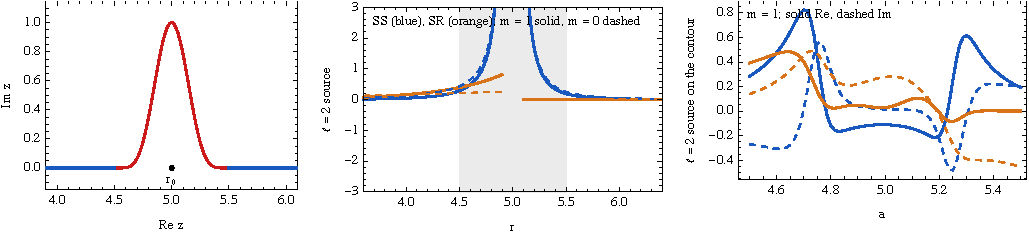
\includegraphics[width=\textwidth]{fig_contour_source.pdf}
\caption{(a) The contour $z=y(a)$. (b) The $\ell=2$ SS (blue) and SR (orange) source modes on the real axis for $m=1$ (solid) and $m=0$ (dashed); the $\delta$ terms are not shown. (c) The continued sources on the contour for $m=1$, real (solid) and imaginary (dashed) parts.}
\label{fig:source}
\end{figure}

\begin{table}[h]
\centering
\caption{The SS source by blended complex-radius angular quadrature, maximum over $\ell\le6$: pointwise relative difference from the closed-form continuation at the 128 contour nodes, and the scaled exterior SS field obtained from the quadrature source by the contour Green's-function quadrature. ``One branch'' is the out-branch alone, without the blend.}
\label{tab:t2}
\footnotesize
\begin{tabular}{llllll}
\toprule
$m$ & pointwise & exterior (quad.) & exterior (closed form) & one branch, pointwise & one branch, exterior\\
\midrule
$\tfrac15$ & $6.5\times10^{-15}$ & $2.0\times10^{-15}$ & $1.7\times10^{-15}$ & $0.07$--$0.09$ & $0.3$--$1.1$\\
$1$ & $7.7\times10^{-15}$ & $6.4\times10^{-16}$ & $6.3\times10^{-16}$ & $0.48$--$0.63$ & $1.8$--$2.7$\\
$0$ & $6.3\times10^{-15}$ & $4.1\times10^{-15}$ & $3.3\times10^{-15}$ & $6\times10^{-16}$ & $5.5\times10^{-15}$\\
\bottomrule
\end{tabular}
\end{table}

\begin{itemize}[leftmargin=*]
\item \emph{Accuracy and node count.} With 80 Gauss nodes per segment (160 evaluations of the three-dimensional source per contour node, 64 residue samples in addition) the blended quadrature reproduces the closed-form continuation of the massive SS source to $8\times10^{-15}$ pointwise and the exterior SS field to $2\times10^{-15}$, the same as the massless case run through the same code ($6\times10^{-15}$, $4\times10^{-15}$) and as the PRD's $1.8\times10^{-14}$. The convergence with the node count is exponential and independent of $m$: $3\times10^{-4}$, $1.3\times10^{-7}$, $3\times10^{-11}$, $7\times10^{-15}$ and $2\times10^{-24}$ pointwise for 32, 48, 64, 80 and 120 nodes per segment, with the exterior field reaching its $10^{-15}$ floor (the 128-node contour quadrature) at 80 nodes (Fig.~\ref{fig:nodes}). The exponential factor $e^{-2m\rho}$, which varies by $e^{-20}$ along the first segment at $m=1$, costs nothing: the integrand is smooth on both segments.
\item \emph{The blend is necessary.} One branch alone, which was sufficient for the massless SS source, is wrong by $7$--$9\%$ pointwise at $m=\tfrac15$ and by $50$--$60\%$ at $m=1$, and gives exterior errors of order one ($0.3$--$2.7$); at $m=0$ the same code gives $6\times10^{-16}$, confirming that the difference between the branches is the real-analytic kink part $2G_{\rm o}$ of Sec.~\ref{sec:ssmodes}, which vanishes without the mass. The residues $A$ agree with the symbolic coefficient of $\rho^{-1}$ to $10^{-30}$.
\item \emph{The same quadrature for SR.} Applied to $2qe^{-m\rho}\PhiR/\rho$ (an entire integrand in $\rho$, so $A=0$ and the blend is the massless one), the quadrature reproduces the closed-form continuation of the SR source, built from the Bessel couplings, to $8\times10^{-16}$ pointwise and the exterior SR field to $1.3\times10^{-16}$.
\end{itemize}

\begin{figure}[t]
\centering
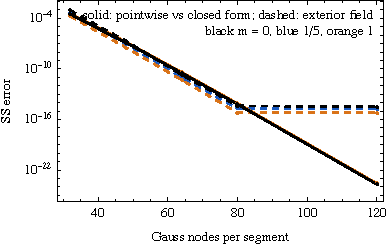
\includegraphics[width=0.55\textwidth]{fig_ss_nodes.pdf}
\caption{Convergence of the SS quadrature with the number of Gauss nodes per segment: pointwise relative error against the closed form (solid) and scaled exterior error (dashed), for $m=0$, $\tfrac15$, $1$.}
\label{fig:nodes}
\end{figure}

\subsection{Consistency of the continued singular mode (T3)}\label{sec:t3}
All numbers in this section come from \code{massive\_stage1\_first\_order.wls} (406 checks, all passed; 8.1~min).
Table~\ref{tab:t3} lists the two consistency conditions for the $\Theta\to H$ singular mode, the residual $E_0$ of Eq.~\eqref{eq:E0} and the corrected mode.

\begin{table}[h]
\centering
\caption{The continued singular mode, $\ell=0$--$6$, $m=\tfrac15,1,0$ (maximum over $\ell$ where a range is given). Condition (i): $\max|\Re\tilde\psi(r+i0)-G_\ell|$ over 17 points on both sides of $r_0$. Condition (ii): real and imaginary parts of $\Lop\tilde\psi-\dext$ on the axis. $E_0(r_0)$ from Eq.~\eqref{eq:E0}. Corrected mode: contour-ODE residual of $\tilde P$ relative to $\max|E_0|$, and $|\tilde P(a_R)-P(a_R)|$ relative to $|P(a_R)|$ (return to the real solution).}
\label{tab:t3}
\footnotesize
\begin{tabular}{lllllll}
\toprule
$m$ & (i) & (ii) real & (ii) imaginary, $\ell=0$ to $6$ & $E_0(r_0)$ & ODE residual & return\\
\midrule
$\tfrac15$ & $<10^{-76}$ & $<10^{-36}$ & $0.54$ to $2.9\times10^4$ & $-0.2000$ & $<10^{-8}$ & $<10^{-12}$\\
$1$ & $<10^{-85}$ & $<10^{-35}$ & $19$ to $6.1\times10^4$ & $-0.2000$ & $<10^{-8}$ & $<10^{-12}$\\
$0$ & $0$ (exact) & $<10^{-36}$ & $0.32$ to $2.8\times10^4$ & $-0.2000$ & $<10^{-8}$ & $<10^{-12}$\\
\bottomrule
\end{tabular}
\end{table}

\begin{itemize}[leftmargin=*]
\item \emph{(i) holds, (ii) fails, exactly as in the massless case.} The real part of the $\Theta\to H$ mode is the mode of the three-dimensional puncture on both sides of $r_0$ to the precision of the arithmetic, and $\Lop\tilde\psi-\dext$ is purely imaginary on the axis. Its size grows quickly with $\ell$ (to $6\times10^4$ at $\ell=6$ for $m=1$), because $J=G^{\rm out}-G^{\rm in}$ grows like $(r/r_0)^{\pm\ell}$ away from $r_0$; at $r_0$ itself $E_0=-1/r_0$ for every $\ell$ and $m$, as Eq.~\eqref{eq:E0} predicts, and the massless $\ell=0$ value $E_0=-1/z$ of PRD App.~C is recovered at $m=0$ to $10^{-25}$.
\item \emph{The corrected mode} $\tilde\psi-\tfrac i\pi P$ satisfies $\Lop\psi^{\rm S}=\dext$ identically and keeps the real part of (i). Its continuation $\tilde P$ along the contour returns to the real $P$ at $a_R$ to $10^{-12}$ relative (the limit of the 30-digit NDSolve at $\ell=6$), confirming that $E_0$ is analytic and that no $2\pi i$ jump occurs. At $m=0$, $\ell=0$ the corrected mode equals $\tilde\psi+\tfrac{i}{2\pi}z$ and has the real part of the massless closed-form $\phi^{\rm S}_0=\psi_p-D_0$ exactly, the imaginary parts differing by a homogeneous solution, as the freedom $i\times$(real homogeneous) of the construction allows.
\item \emph{DSolve.} For the massive operator DSolve returns closed forms: exponential integrals ${\rm Ei}(\pm m(r-r_0))$ for $\ell=0$, and sinh and cosh in\-te\-grals times spherical Bessel functions for $\ell=2$. Evaluated from above, $\Re\psi_p(r+i0)-G_\ell$ is a homogeneous solution $\alpha u_\ell+\beta v_\ell$ on both sides (fit residual below $10^{-38}$), with $(\alpha,\beta)=(1.84,34.0)$ at $m=\tfrac15$ and $(0.034,371)$ at $m=1$ for $\ell=0$, and $\alpha=0.034$, $0.0039$ with $\beta<10^{-36}$ for $\ell=2$. The pattern of the massless App.~C persists: an anti-physical Green's function at $\ell=0$ and a one-sided one at $\ell\ge2$ (compare $\alpha=r_0^{1-\ell}/(2\ell+1)=0.04$ at $m=0$), so the DSolve particular solution cannot be used as the singular mode without the offset correction here either.
\item \emph{Residual solves on the contour} (Stage~1, table \code{massive\_stage1\_\allowbreak residual\_\allowbreak solves.csv}). With the test regular field $u_\ell(r)/u_\ell(r_0)$ injected at $r=1$ and $S_{\rm eff}=\kappa_\ell(\dext-\Lop\phi^{\rm P})$, the exterior regular field is exact to $4.6\times10^{-18}$ (scaled) for every puncture and every $\ell\le6$ and $m$. With the $\Theta\to H$ puncture the residual on the contour carries an $O(1)$ shadow ($0.12$--$1$ of the field, equal to the continued $-\tfrac i\pi\kappa_\ell\tilde P$ to $10^{-19}$); with the corrected puncture it carries none ($<3\times10^{-18}$); with the truncated punctures $\PhiP_n$ it equals the closed form $\tilde\phi^{\rm R}+\kappa_\ell(\tilde f-\tilde\phi^{\rm P}_n)$ to $3\times10^{-18}$ and its shadow is the truncation remainder, $10^{-3}$--$3\times10^{-2}$ at $m=\tfrac15$ and $10^{-2}$--$0.4$ at $m=1$ for $\ell\le2$ (the puncture is used without a window, so for $mr_0=5$ its polynomial tail is large at $\rho\sim2r_0$).
\item \emph{Smoothness of the residual.} For $n=1,3,5$ and $\ell'=0,2,5$ the modes of $\Phi_1-\PhiP_n$ at $r_0$ have continuous derivatives through order $n+3$ ($<10^{-80}$) and a jump in the $(n+4)$th, as predicted in Sec.~\ref{sec:trunc}: the modes are $C^{n+3}$ and the three-dimensional residual $C^{n+1}$.
\end{itemize}

\subsection{Exact puncture: the exterior field}\label{sec:exact}
\code{massive\_stage3\_\allowbreak contour.wls} part C (328 checks pass in the whole stage; 39.5~min).
With the exact puncture $qe^{-m\rho}/\rho$ the SS and SR sources are solved by three-region NDSolve solves (real axis, contour, real axis) with the physical conditions and the closed-form contour sources, RR on the real line; the sources are tabulated on piecewise Chebyshev interpolants (40 contour pieces, $2\times16$ real pieces, 24 nodes each) as in the massless Stage~8.
Table~\ref{tab:exact} and Fig.~\ref{fig:rec} give the result.

\begin{table}[h]
\centering
\caption{Exact puncture: scaled exterior errors, maximum over $\ell\le6$, each piece scaled by its own reference and SS$+$SR by $\max|{\rm SS}+{\rm SR}|$; point-supported fit $|\alpha|+|\beta|$ (monopole and dipole at $\x_0$, one point in each exterior region); and the pointwise real-line SR without its $\delta$ term (negative control) before and after adding $c_\ell G_\ell(r,r_0)$.}
\label{tab:exact}
\footnotesize
\begin{tabular}{lllllllll}
\toprule
$m$ & SS & SR & RR & SS$+$SR & fit SS & fit SR & SR, no $\delta$ & $+c_\ell G$\\
\midrule
$\tfrac15$ & $5.1\,10^{-18}$ & $5.4\,10^{-18}$ & $2.1\,10^{-20}$ & $2.6\,10^{-18}$ & $8.3\,10^{-18}$ & $2.6\,10^{-18}$ & $1.9$--$4.3$ & $1.5\,10^{-17}$\\
$1$ & $4.3\,10^{-17}$ & $8.7\,10^{-17}$ & $2.3\,10^{-20}$ & $7.0\,10^{-17}$ & $1.5\,10^{-16}$ & $4.8\,10^{-16}$ & $1.1$--$1.3$ & $1.0\,10^{-16}$\\
$0$ & $5.7\,10^{-18}$ & $4.6\,10^{-18}$ & $1.7\,10^{-20}$ & $2.5\,10^{-18}$ & $9.4\,10^{-18}$ & $2.9\,10^{-18}$ & $1.8$--$6.3$ & $1.2\,10^{-17}$\\
\bottomrule
\end{tabular}
\end{table}

\begin{figure}[t]
\centering
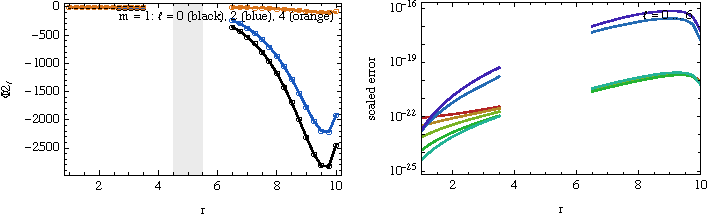
\includegraphics[width=0.95\textwidth]{fig_recovered_modes.pdf}
\caption{Left: recovered exterior modes $\Phi_{2,\ell}$ (circles) against the reference (lines) for $m=1$, $\ell=0,2,4$. Right: scaled error against $r$ for $\ell=0$--$6$.}
\label{fig:rec}
\end{figure}

\begin{itemize}[leftmargin=*]
\item \emph{Seventeen digits with Bessel functions.} The exterior SS and SR fields are recovered to $5\times10^{-18}$ at $m=\tfrac15$ and $9\times10^{-17}$ at $m=1$, against $3\times10^{-18}$ in the massless PRD; the $m=1$ figure is the 30-digit NDSolve evaluating Bessel functions, not the method. The massless case run through the same code gives $6\times10^{-18}$.
\item \emph{No spurious worldline terms (T3 (iv)).} The fit of the SS and SR errors to the physical responses of a monopole and a dipole at $\x_0$ gives $|\alpha|+|\beta|\le1.5\times10^{-16}$ and $4.8\times10^{-16}$ (massless: $1.1\times10^{-18}$), while the positive control, a unit $\delta^3$ added to the SS contour source as $Y_\ell(0)\dext/r_0^2$, is detected with $\alpha=-0.0795774715459=-1/4\pi$ to twelve digits and $\beta<10^{-17}$ for all three masses.
\item \emph{The $\delta$ content is essential and is produced by the contour.} Solving the pointwise SR source on the real line, which drops the $\delta$ term, is wrong by factors $1.1$--$6.3$; adding $c_\ell G_\ell(r,r_0)$ with the coefficient of Eq.~\eqref{eq:deltas} restores the field to $10^{-16}$. The SR $\delta$ coefficient is $c_\ell=-0.2127$, $-0.3684$, $-0.4756$, $-0.5627$, $-0.6381$, $-0.7054$, $-0.7669$ for $\ell=0$--$6$ at $m=1$ (and at $m=\tfrac15$ and $0$), the massless values, as predicted; the SS $\delta$ coefficient $4\pi mq^2Y_\ell(0)/r_0^2$ is $0.1418$, $0.2456$, $0.3171$, $0.3752$, $0.4254$, $0.4703$, $0.5113$ at $m=1$ and one fifth of that at $m=\tfrac15$.
\item \emph{Shadows.} The imaginary parts of the SS and SR contour solutions at $a_R$ are $0.08$--$0.38$, as in the massless case, and harmless.
\end{itemize}

\subsection{Truncated punctures: convergence with the coupled-mode cutoff (T1)}\label{sec:t1}
All numbers come from \code{massive\_stage4\_\allowbreak convergence.wls} (203 checks pass; 26.4~min), with the error scaled by the size of the SS$+$SR reference and maximised over $\ell\le6$ and the exterior grid.
Figure~\ref{fig:conv} and Table~\ref{tab:t1} summarise the hybrid split.

\begin{figure}[t]
\centering
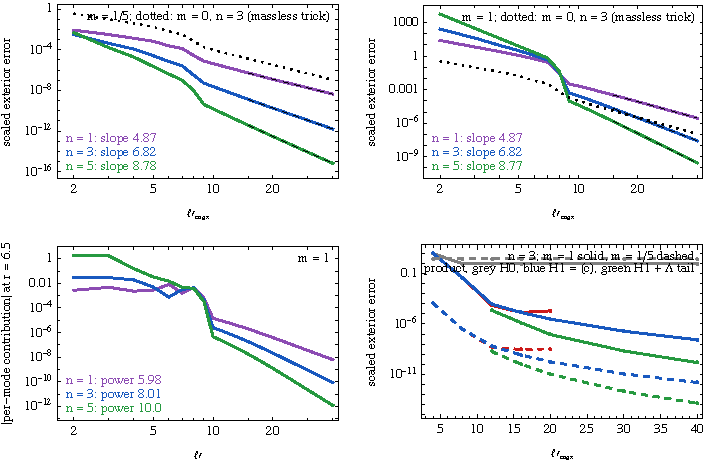
\includegraphics[width=0.95\textwidth]{fig_convergence.pdf}
\caption{Hybrid split, $k=0$. Top: scaled exterior error against $\lpm$ for $n=1,3,5$ at $m=\tfrac15$ (left) and $m=1$ (right), with the fitted slopes (dashed) and the massless trick puncture at $m=0$, $n=3$ (dotted). Bottom left: per-mode contributions at $r=6.5$, $m=1$. Bottom right: routes for $n=3$: product (red), H0 (grey), H1 $=$ (c) (blue), H1 with the one-term $\Lambda$ tail (green); $m=1$ solid, $m=\tfrac15$ dashed.}
\label{fig:conv}
\end{figure}

\begin{table}[h]
\centering
\caption{Convergence of the hybrid split (H1, $k=0$) with the coupled-mode cutoff. Slopes are least-squares fits of $\log$ error against $\log\lpm$ over $20\le\lpm\le40$; the per-mode power is fitted to the contributions at $r=6.5$ for $25\le\ell'\le40$. Expected values in brackets: $n+4$ and $n+5$ for the massive punctures, $n+2$ and $n+3$ for the massless trick. The last column gives the error scaled by the total field, the massless convention.}
\label{tab:t1}
\footnotesize
\begin{tabular}{llllllll}
\toprule
$m$ & $n$ & slope (exp.) & per-mode (exp.) & $\lpm=12$ & 20 & 40 & $40$, by $\max|\Phi_2|$\\
\midrule
$\tfrac15$ & 1 & 4.87 (5) & 6.01 (6) & $1.7\times10^{-6}$ & $1.3\times10^{-7}$ & $4.3\times10^{-9}$ & $4.0\times10^{-9}$\\
$\tfrac15$ & 3 & 6.82 (7) & 8.02 (8) & $6.6\times10^{-9}$ & $1.8\times10^{-10}$ & $1.6\times10^{-12}$ & $1.5\times10^{-12}$\\
$\tfrac15$ & 5 & 8.78 (9) & 10.1 (10) & $2.9\times10^{-11}$ & $3.0\times10^{-13}$ & $6.7\times10^{-16}$ & $6.3\times10^{-16}$\\
$1$ & 1 & 4.87 (5) & 5.98 (6) & $9.5\times10^{-4}$ & $8.4\times10^{-5}$ & $2.9\times10^{-6}$ & $2.9\times10^{-6}$\\
$1$ & 3 & 6.82 (7) & 8.01 (8) & $9.0\times10^{-5}$ & $3.0\times10^{-6}$ & $2.7\times10^{-8}$ & $2.7\times10^{-8}$\\
$1$ & 5 & 8.77 (9) & 10.0 (10) & $9.7\times10^{-6}$ & $1.2\times10^{-7}$ & $2.8\times10^{-10}$ & $2.8\times10^{-10}$\\
$0$ (trick) & 3 & 4.87 (5) & 6.01 (6) & $3.9\times10^{-5}$ & $3.3\times10^{-6}$ & $1.1\times10^{-7}$ & $1.1\times10^{-7}$\\
\bottomrule
\end{tabular}
\end{table}

\begin{itemize}[leftmargin=*]
\item \emph{The rates are those of a $C^{n+1}$ residual.} The fitted slopes $4.87$, $6.82$, $8.78$ and per-mode powers $6.0$, $8.0$, $10.0$ for $n=1,3,5$ are the predicted $n+4$ and $n+5$ to the same shortfall ($0.1$--$0.2$ in the slope) that the massless fits showed against $n+2$ and $n+3$; they are identical at $m=\tfrac15$ and $m=1$, as they should be, since only the smoothness of the residual at $\x_0$ enters. The massless trick puncture run through the same code at $m=0$ reproduces the massless Stage~12b exactly: slope $4.87$, per-mode power $6.01$, and errors $3.90\times10^{-5}$, $3.27\times10^{-6}$, $1.11\times10^{-7}$ at $\lpm=12,20,40$ (massless: $4.87$, $6.01$, and the same three numbers to three digits).
\item \emph{The prefactor is set by $mr_0$.} Between $m=\tfrac15$ and $m=1$ the error grows by $6\times10^2$ ($n=1$) to $4\times10^5$ ($n=5$) at $\lpm=40$, the ratio of the coefficients $m^{n+3}/(n+3)!$ of the first non-smooth term; for $mr_0=5$ a truncation at $\rho^5$ gives $3\times10^{-10}$ at $\lpm=40$.
\item \emph{H1 equals the mode-truncation error (c) for every $n$ and $\lpm$}, because Part~1 carries the whole $\delta$ term of the truncated SR source ($<10^{-46}$ relative) and the truncated RR source has none; the $\delta$ coefficients of the truncated sources approach $c_\ell$ as $\Pres_M(\x_0)\to\PhiR(\x_0)$ (to $3\times10^{-5}$ at $n=1$, $m=1$, $\lpm=40$, and $10^{-8}$ at $n=5$).
\item \emph{H0 fails at order one}, $2.76$ at $m=\tfrac15$ and $0.91$ at $m=1$ (scaled), independently of $\lpm$: the missing $c_\ell\delta$ term.
\item \emph{The product route} follows (c) and then turns up: at $m=1$, $n=3$ its error is $6.8\times10^{-5}$, $1.4\times10^{-5}$, $2.0\times10^{-5}$ at $\lpm=12,16,20$ against $9.0\times10^{-5}$, $1.4\times10^{-5}$, $3.0\times10^{-6}$ for H1, and at $n=5$ it is $1.8$ times H1 at $\lpm=20$; at $m=\tfrac15$, $n=3$ the minimum is at $\lpm=16$. The shadow contribution of the coupled mode $\ell'$ grows by $1.129$ per unit $\ell'$ near $\ell'=30$ for $R=\tfrac12$ and $1.062$ for $R=\tfrac14$ at both masses ($1.132$ and $1.062$ with the massless puncture; PRD App.~D: $1.12$ and $1.06$), i.e.\ still $1+R/r_0$ times a slowly varying power: the Bessel modes grow across the tube like the powers for $\ell'\gg mr$.
\item \emph{Tail acceleration} with two terms of Upton's $\Lambda_{\ell',0,-p}$, $p=n+5$, gains a factor $16$--$29$ at $\lpm=20$, $160$--$690$ at $30$ and $3\times10^3$--$10^4$ at $40$; the one-term fit gains $14$--$38$ at $20$ and $3$--$5$ at $\lpm=12$, where the two-term fit still makes things worse, as in the massless case.
\item \emph{Error against $r$.} With the physical conditions the error is largest next to the tube and decays outwards on both sides ($m=1$, $n=3$, $\lpm=20$: $1.3\times10^{-5}$ in $[3.5,4.5]$, $5.0\times10^{-6}$ in $[5.5,6.5]$, $2.1\times10^{-6}$ in $[6.5,10]$).
\end{itemize}

\subsection{Shadow growth, Cauchy step and noise}\label{sec:misc}
\paragraph{Cauchy step.}
For $n=3$, $\lpm=8$ and $20$, $\ell=2$ and $6$, the actual contour solves of the H1 and H0 sources (Part~2 Cauchy-continued with the massless Stage-8 machinery, Part~1 in closed form) were compared with the distributional real-line response at $a_R$.
The difference equals the predicted $\delta$ miss ($-(g_{\rm SR}-g_{\rm P1})\{g_0,g_1\}$, zero for H1) to $10^{-18}$ at $m=\tfrac15$ and $3\times10^{-15}$ at $m=1$ relative to $|c_\ell G|$, and propagated with the physical conditions the Cauchy step contributes at most $3.5\times10^{-17}$ ($m=\tfrac15$) and $2.4\times10^{-15}$ ($m=1$) to the scaled exterior error, below $2\times10^{-7}$ of the H1 error in every case and below $10^{-9}$ except at $\lpm=20$, $\ell=6$.
The $m=1$ values are larger than the massless $1.3\times10^{-16}$ because the Bessel functions are evaluated at 30 digits inside NDSolve.

\paragraph{Shadow growth.}
See the product-route item of Sec.~\ref{sec:t1}: $1.129$ and $1.062$ per coupled mode for $R=\tfrac12$ and $\tfrac14$, unchanged from the massless $1.132$, $1.062$.

\paragraph{Noise.}
With $10^{-8}$ relative Gaussian noise on the SS mode samples, the noise-induced exterior error (the systematic part cancels in the difference) is $5\times10^{-9}$--$2.5\times10^{-8}$ for 64 contour nodes, against $1.3\times10^{-2}$--$8.6\times10^{-2}$ for 112 samples on a real-axis grid graded towards $r_0$ (Gauss panels with ratio $\tfrac15$ down to $3\times10^{-5}$ from the particle, as needed to resolve the $\Delta r^{-2}$ singularity): the real-axis route is $1$--$5\times10^6$ times more sensitive, for every $\ell\le6$ and for $m=0,\tfrac15,1$ alike. The ratio is larger than the massless $10^2$--$3\times10^5$ only because the graded grid here samples closer to $r_0$, where the samples are amplified by $\Delta r^{-2}$; the contour's own sensitivity, a factor $0.5$--$2.5$ on the noise, is the same as the massless one.

\section{What carried over and what did not}\label{sec:carry}
\paragraph{What carried over unchanged.}
\begin{itemize}[leftmargin=*]
\item The contour, the extended delta function, the $\Theta\to H$ blend of kinked modes and the linear-solve property: every exterior error in this note is the Green's-function response of its error source, exactly as in the massless Stage~12b, and the actual contour solves agree with that decomposition at the level of the Cauchy step.
\item The two consistency conditions on the continued singular mode, with the same outcome: (i) holds for the $\Theta\to H$ blend, (ii) fails by a purely imaginary residual that is harmless for the exterior field but puts an $O(1)$ shadow on the residual, and the corrected mode fixes it. The offset structure of DSolve's particular solutions is also the same.
\item The $\rho$-substitution of the angular quadrature: a single fixed pole at $\rho=0$ and the two-segment path, with the same node count (64--80 per segment) for the same accuracy, although the integrand now contains $e^{-2m\rho}$.
\item The hybrid split with $k=0$: Part~1 carries the whole SR $\delta$ term for every truncation order and every $\lpm$, H1 equals the mode-truncation error, H0 fails by the missing $\delta$, and the product route turns up when the shadows of the coupled modes grow.
\item The physical boundary conditions as Robin conditions at the ends of the domain, with the Bessel logarithmic derivatives in place of $\ell/r$ and $-(\ell+1)/r$, and the zero-data-plus-$\alpha u_\ell$ construction of the three-region solve.
\item The $\delta$ coefficient of the SR source, $c_\ell=-4\pi q\PhiR(\x_0)Y_\ell(0)/r_0^2$, is literally unchanged, because the derivative jump of the massive Coulomb mode is $m$-independent.
\end{itemize}

\paragraph{What did not carry over, or had to be added.}
\begin{itemize}[leftmargin=*]
\item \emph{Both branches of the SS quadrature are needed.} The SS source modes have kinks as well as a logarithm, so one branch no longer has the correct real part on both sides of $r_0$; the undifferentiated modes must be blended with $H$ before the ladder, and the blend must put the logarithm of the in-branch on the same side of the cut as the out-branch (the residue correction $i\pi A$ of Eq.~\eqref{eq:blend}). The canonical (from-above) in-branch, which is the right object for everything else, is the wrong partner for the blend.
\item \emph{The SS source carries a $\delta$ term}, $4\pi mq^2Y_\ell(0)/r_0^2$, from the constant $-mq$ in the local series of the singular field. It is generated on the contour by the $H'$ terms of the blend and must be kept in any real-axis treatment of the massive SS source.
\item \emph{The residual of a truncated puncture is two orders smoother than the massless trick suggested}, because the first omitted term is an even power of $\rho$. The convergence rates are $\lpm^{-(n+4)}$, not $\lpm^{-(n+2)}$, so the comparison between truncation orders in the massless test ($n$ and $n+2$) corresponds to $n$ and $n+2$ here as well, but with a two-order offset in the exponent.
\item \emph{The regular field grows exponentially}, $\PhiR\sim e^{mr}/r$, so at $mr_0=5$ the RR piece dominates the total second-order field by five orders of magnitude at $r=10$ and the errors have to be scaled piece by piece.
\item \emph{The closed-form modes with exponential integrals need branch care at both end points.} The term ${\rm Ei}(-2m(r+r_0))$ sits exactly on Mathematica's branch cut for real $r$ and jumps by $-i\pi$ as soon as $\Im z>0$; it has to be written through the entire part ${\rm Ei}(w)-\gamma-\log w$ of the exponential integral.
\item \emph{The truncated puncture without a window is large far from the particle} at $mr_0=5$. This inflates the shadows of the product route, and the $\rho^k$ modes at large $L$ have to be evaluated from 200-digit input because about 100 digits cancel at $\rho=r+r_0$; neither affects the hybrid route.
\end{itemize}

\section{Limitations}\label{sec:limits}
\begin{itemize}[leftmargin=*]
\item The model is static, scalar and flat; the mass adds non-polynomial homogeneous solutions and an infinite local series for the singular field, but no $m$-modes, two-dimensional angular integrals, window functions or $\ln\rho$ terms in the puncture.
\item The exact reference is numerical (Green's-function quadrature of closed-form mode sources) rather than closed form; its accuracy, $10^{-18}$ or better, is established by cross-checks rather than by an identity, and it sets the floor of the exact-puncture results.
\item The truncated puncture is used everywhere without a window function, as in the massless test. With $mr_0=5$ its polynomial tail is large at $\rho\sim2r_0$; a windowed puncture, as used in gravity, would reduce the size of the residual far from the particle (not its smoothness at the particle, which sets the convergence rate).
\item At $m=1$ the exponentially growing regular field makes RR dominate the total field; the errors of the contour pieces are quoted relative to the size of those pieces.
\item The corrected singular mode is obtained by integrating an ODE rather than in closed form; DSolve's closed forms carry homogeneous offsets and were not used.
\item The noise test compares only the noise-induced parts of the two routes; the systematic accuracy of a real-axis finite-part integration of the massive SS source (which would also need the new $\delta$ term) was not implemented.
\end{itemize}

\section{Reproducibility}\label{sec:repro}
\begin{sloppypar}
The implementation is the folder \code{Massive scalar/Mathematica/}: the package \code{ContourMassive.wl} (a self-contained adaptation of the massless \code{ContourSecondOrder.wl}) and four stage scripts, each printing \code{PASS}/\code{FAIL} against stated tolerances and ending with a summary.
\begin{itemize}[leftmargin=*]
\item \code{massive\_stage1\_\allowbreak first\_\allowbreak order.wls}: first order, T3 (i)--(iii); 406 checks; 8.1~min.
\item \code{massive\_stage2\_\allowbreak reference.wls}: the exact reference and its cross-checks; the $\delta$ coefficients; 192 checks; 3.2~min. It writes the files \code{results/\allowbreak massive\_\allowbreak reference\_\allowbreak m*.mx}, which Stages 3 and 4 read (and recompute if missing or invalid).
\item \code{massive\_stage3\_\allowbreak contour.wls}: T2, the exact-puncture solves, T3 (iv), noise, figures; 328 checks; 39.5~min.
\item \code{massive\_stage4\_\allowbreak convergence.wls}: T1, routes, tail acceleration, Cauchy step, shadow growth, the $m=0$ comparison; 203 checks; 26.4~min.
\end{itemize}
\code{run\_all.sh} runs the four stages (about 80 minutes on a 12-core Apple-silicon Mac with Mathematica 14.3) and builds this note; the argument \code{smoke} runs reduced versions in about ten minutes.
Every table of this note is in the files \code{results/\allowbreak massive\_\allowbreak stage*\_\allowbreak summary.md} with the CSVs behind it; every figure has a CSV beside it in \code{figures/}; the check lists are the files \code{results/\allowbreak massive\_\allowbreak stage*\_\allowbreak checks.csv} and the logs are in \code{results/logs/}.
\code{Mathematica/README.md} documents the conventions and all results, and \code{CHANGELOG.md} has one line per stage.
\end{sloppypar}

\end{document}
